
%(BEGIN_QUESTION)
% Copyright 2006, Tony R. Kuphaldt, released under the Creative Commons Attribution License (v 1.0)
% This means you may do almost anything with this work of mine, so long as you give me proper credit

Complete the calibration table for this flow-measuring loop, consisting of an orifice plate, $\Delta$P transmitter, square root extractor, and indicator.  Assume the following instrument ranges:

$$\includegraphics[width=15.5cm]{i00048x01.eps}$$

\begin{itemize}
\item{} FE: 0-750 GPM, 0-100 "W.C. $\Delta$P
\item{} FT: 0-100 "W.C. in, 4-20 mA out (linear)
\item{} FY: 4-20 mA in and out (square-root)
\item{} FI: 4-20 mA in, 0-750 GPM indication
\end{itemize}

% No blank lines allowed between lines of an \halign structure!
% I use comments (%) instead, so that TeX doesn't choke.

$$\vbox{\offinterlineskip
\halign{\strut
\vrule \quad\hfil # \ \hfil & 
\vrule \quad\hfil # \ \hfil & 
\vrule \quad\hfil # \ \hfil & 
\vrule \quad\hfil # \ \hfil & 
\vrule \quad\hfil # \ \hfil & 
\vrule \quad\hfil # \ \hfil \vrule \cr
\noalign{\hrule}
%
% First row
Flow rate & Percent of & Orifice $\Delta$P & FT output & FY output & FI indication \cr
%
% Another row
(GPM) & max. flow (\%) & ("W.C.) & signal (mA) & signal (mA) & (GPM) \cr
%
\noalign{\hrule}
%
% Another row
0 & 0 &   &   &   & 0 \cr
%
\noalign{\hrule}
%
% Another row
  & 10 &   &   &   &  \cr
%
\noalign{\hrule}
%
% Another row
  & 25 &   &   &   &  \cr
%
\noalign{\hrule}
%
% Another row
375 & 50 &   &   &   & 375 \cr
%
\noalign{\hrule}
%
% Another row
  & 75 &   &   &   &  \cr
%
\noalign{\hrule}
%
% Another row
  & 90 &   &   &   &  \cr
%
\noalign{\hrule}
%
% Another row
750 & 100 &   &   &   & 750 \cr
%
\noalign{\hrule}
} % End of \halign 
}$$ % End of \vbox

\vfil

\underbar{file i00048}
\eject
%(END_QUESTION)





%(BEGIN_ANSWER)

This is a graded question -- no answers or hints given!

%(END_ANSWER)





%(BEGIN_NOTES)

% No blank lines allowed between lines of an \halign structure!
% I use comments (%) instead, so that TeX doesn't choke.

$$\vbox{\offinterlineskip
\halign{\strut
\vrule \quad\hfil # \ \hfil & 
\vrule \quad\hfil # \ \hfil & 
\vrule \quad\hfil # \ \hfil & 
\vrule \quad\hfil # \ \hfil & 
\vrule \quad\hfil # \ \hfil & 
\vrule \quad\hfil # \ \hfil \vrule \cr
\noalign{\hrule}
%
% First row
Flow rate & Percent of & Orifice $\Delta$P & FT output & FY output & FI indication \cr
%
% Another row
(GPM) & max. flow (\%) & ("W.C.) & signal (mA) & signal (mA) & (GPM) \cr
%
\noalign{\hrule}
%
% Another row
0 & 0 & 0 & 4 & 4 & 0 \cr
%
\noalign{\hrule}
%
% Another row
75  & 10 & 1 & 4.16 & 5.6 & 75 \cr
%
\noalign{\hrule}
%
% Another row
187.5  & 25 & 6.25 & 5 & 8 & 187.5 \cr
%
\noalign{\hrule}
%
% Another row
375 & 50 & 25 & 8 & 12 & 375 \cr
%
\noalign{\hrule}
%
% Another row
562.5 & 75 & 56.25 & 13 & 16 & 562.5 \cr
%
\noalign{\hrule}
%
% Another row
675 & 90 & 81 & 16.96 & 18.4 & 675 \cr
%
\noalign{\hrule}
%
% Another row
750 & 100 & 100 & 20 & 20 & 750 \cr
%
\noalign{\hrule}
} % End of \halign 
}$$ % End of \vbox

Converting percentage values into flow rates is easy: simply multiply each percentage by the maximum (URV) flow rate.

\vskip 10pt

Converting percentage values into differential pressure values is a little trickier.  Since the orifice plate is inherently nonlinear -- generating differential pressure proportional to the {\it square} of the flow rate -- we must take the percentage of flow and then square that percentage to arrive at a percentage of DP.  This new (squared) percentage value is then multiplied by the URV of the pressure range to calculate DP.

\vskip 10pt

The flow transmitter itself is linear, and so it simply takes the sensed DP and converts it linearly to a milliamp output signal.

\vskip 10pt

The square root ``extractor'' (relay) takes in the transmitter's milliamp signal, square-roots that signal percentage, then generates its own milliamp signal representing percentage of flow.  The end-result is that the relay's milliamp signal is linear to actual flow rate.

%INDEX% Calibration: table, flow transmitter
%INDEX% Measurement, flow: calibration table

%(END_NOTES)


